\subsection{Trash}
%%% 6-by-6 3 agents r3 no obs
\begin{figure}[H]
  \centering
  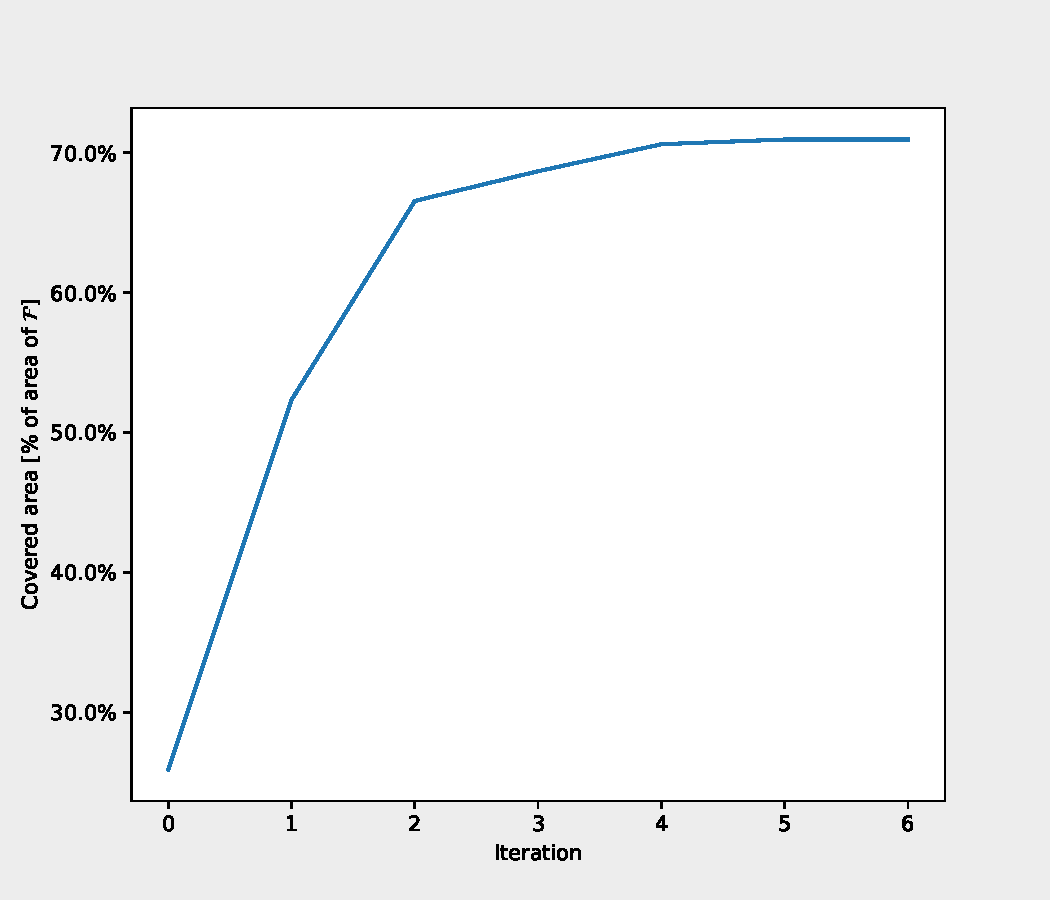
\includegraphics[width=.75\textwidth]{figs/6_by_6_no_obs_3_agnts_area_traj.pdf}
  \caption{Percentage covered for rectangular environment.}
  \label[fig]{local_coverage_example}
\end{figure}
\begin{figure}[H]
  \centering
  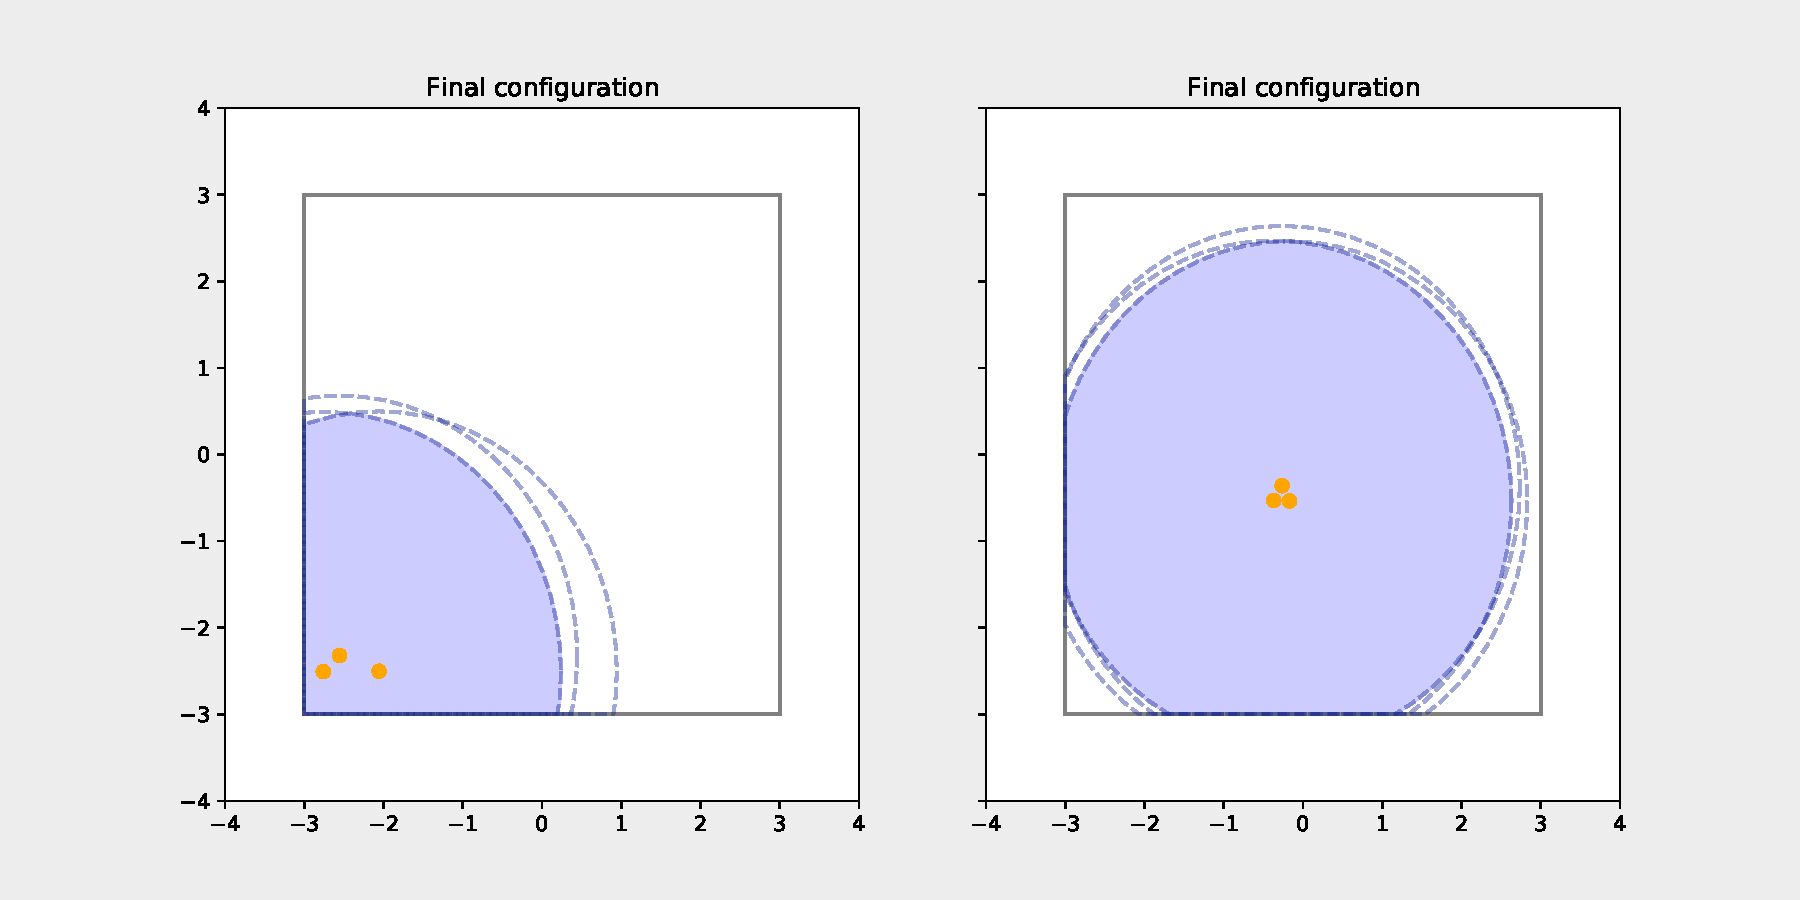
\includegraphics[width=.75\textwidth]{figs/6_by_6_no_obs_3_agnts_distr.pdf}
  \caption{Inital and final position of agents in rectangular environment.}
  \label[fig]{local_coverage_example}
\end{figure}

%%% 6-by-6 10 agents r3 no obs
\begin{figure}[H]
  \centering
  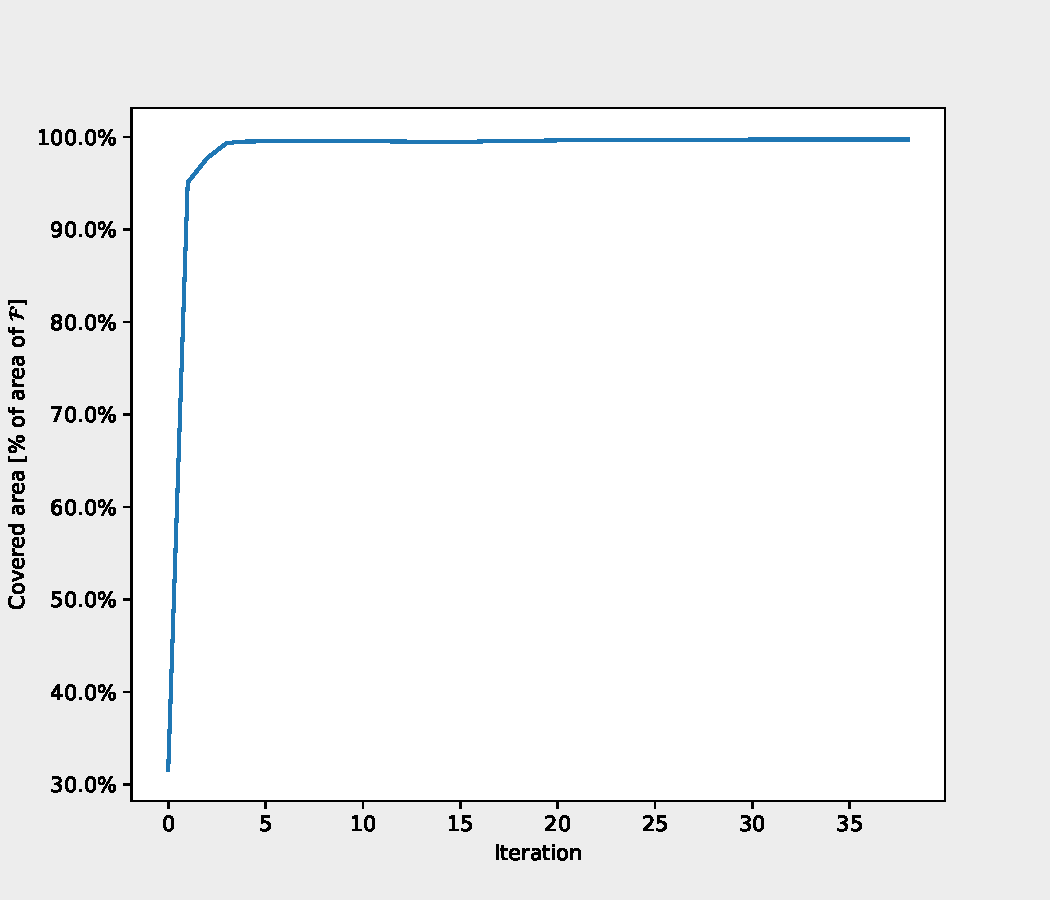
\includegraphics[width=.75\textwidth]{figs/6_by_6_no_obs_10_agnts_area_traj.pdf}
  \caption{Percentage covered  for rectangular environment with rectangular central obstacle.}
  \label[fig]{local_coverage_example}
\end{figure}
\begin{figure}[H]
  \centering
  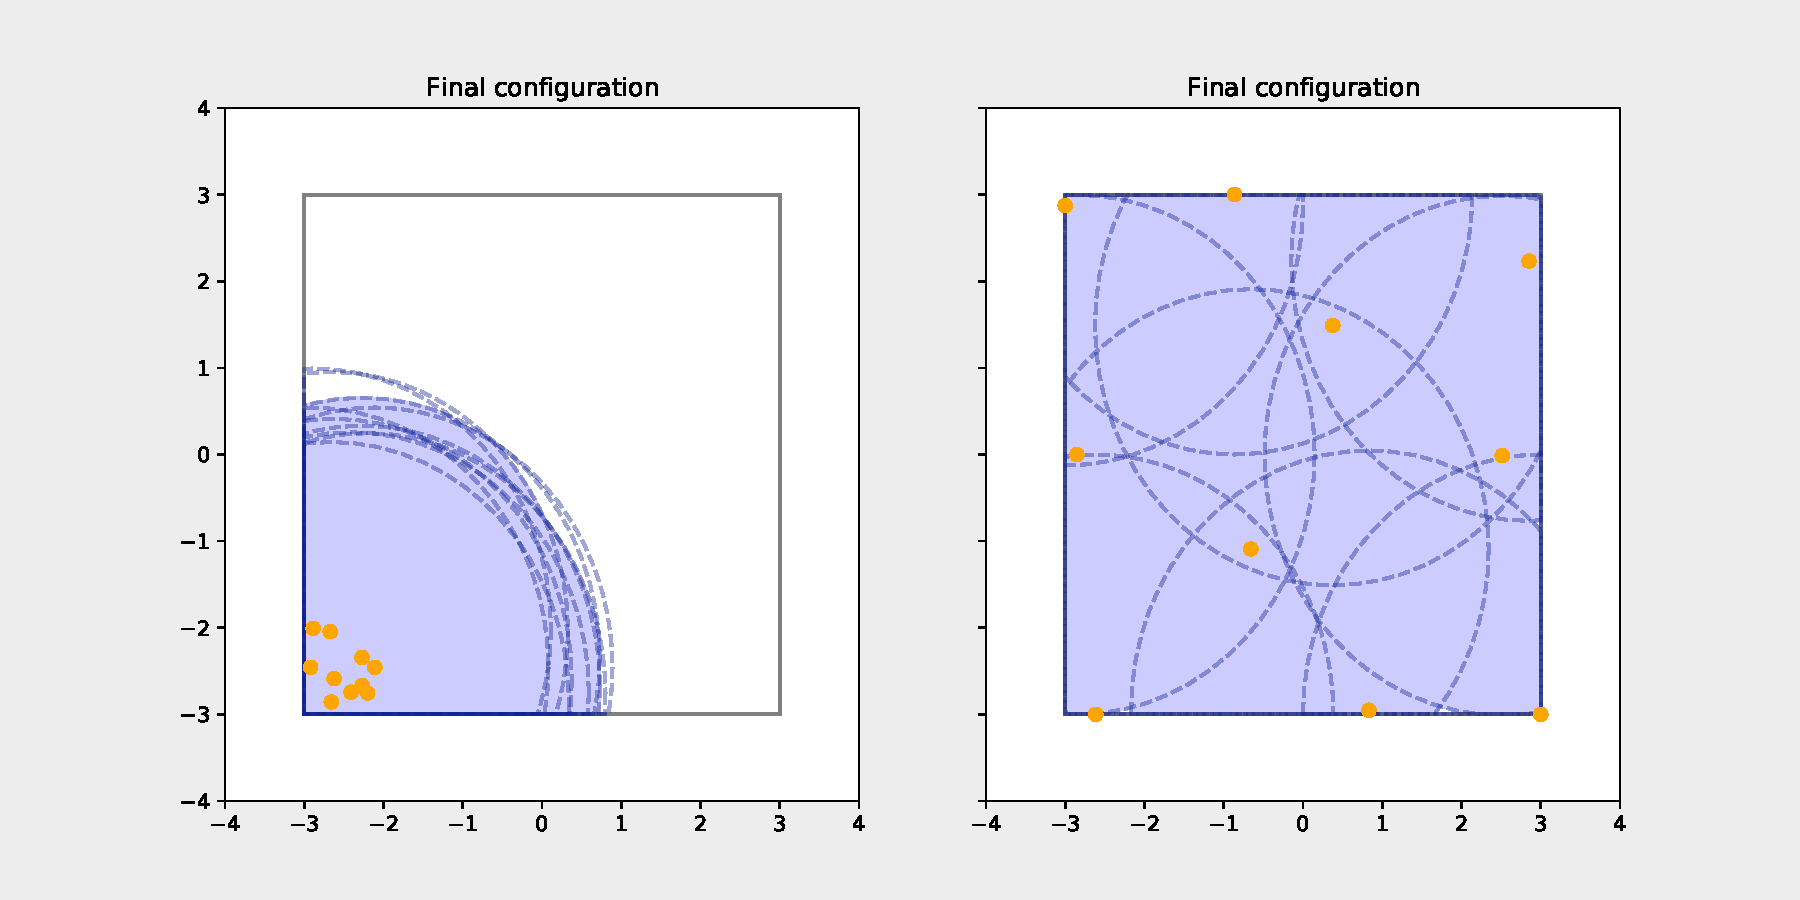
\includegraphics[width=.75\textwidth]{figs/6_by_6_no_obs_10_agnts_distr.pdf}
  \caption{Inital and final position of agents in rectangular environment with rectangular central obstacle.}
  \label[fig]{local_coverage_example}
\end{figure}


%%% 2-by-2 Three agents r3
\begin{figure}[H]
  \centering
  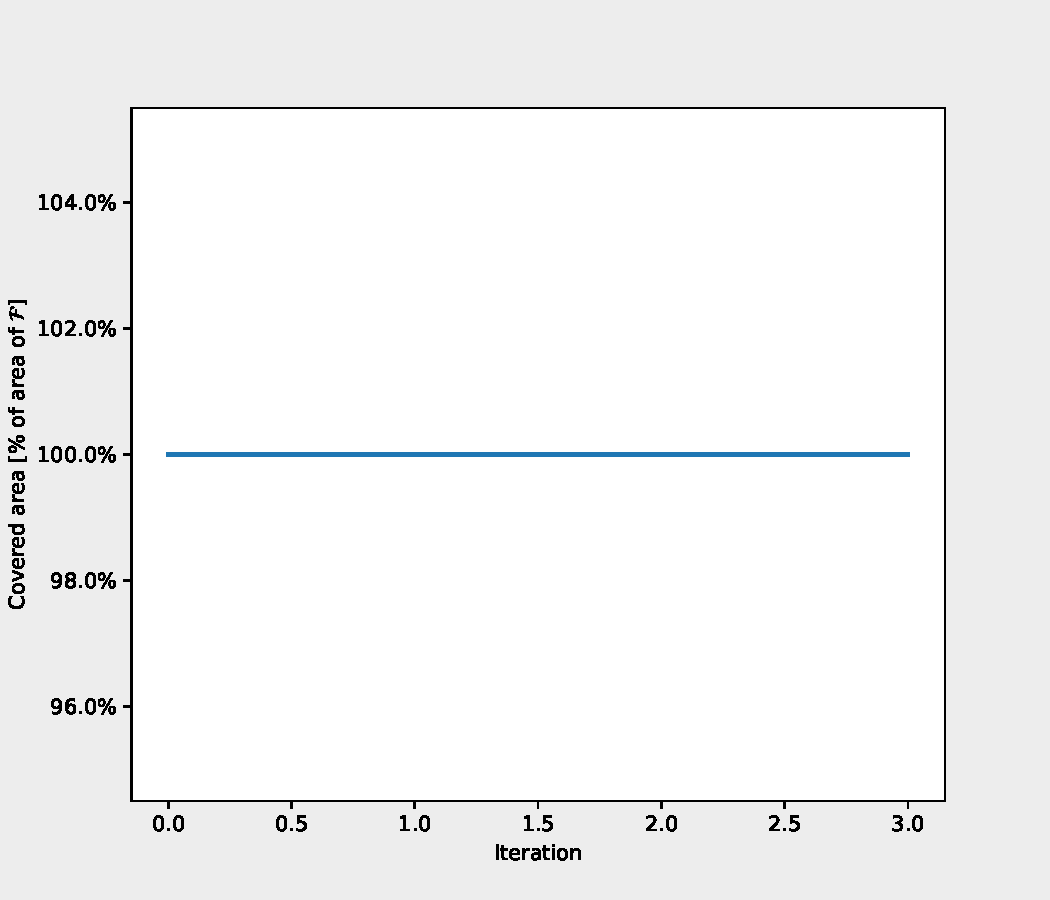
\includegraphics[width=.75\textwidth]{figs/1_by_1_no_obs_3_agnts_area_traj.pdf}
  \caption{Percentage covered  for rectangular obstacle-less environment. }
  \label[fig]{local_coverage_example}
\end{figure}
\begin{figure}[H]
  \centering
  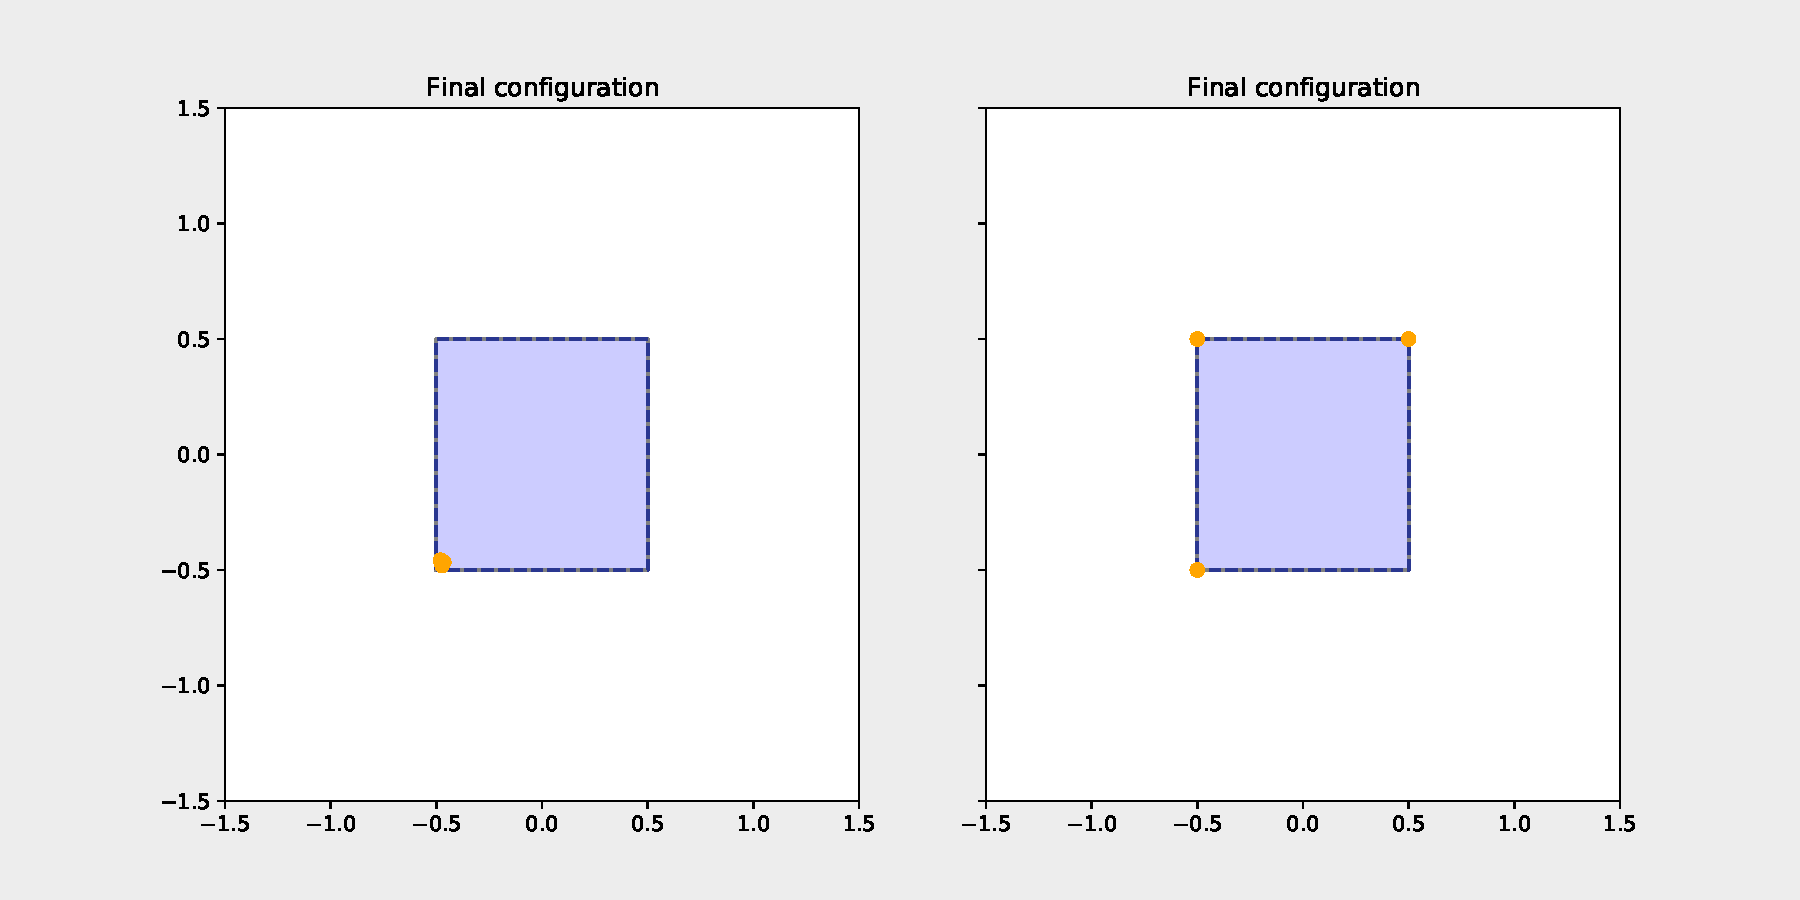
\includegraphics[width=.75\textwidth]{figs/1_by_1_no_obs_3_agnts_distr.pdf}
  \caption{Inital and final position of agents in rectangular obstacle-less environment.}
  \label[fig]{local_coverage_example}
\end{figure}

%%% 2-by-2 Three agents r3 center obs
\begin{figure}[H]
  \centering
  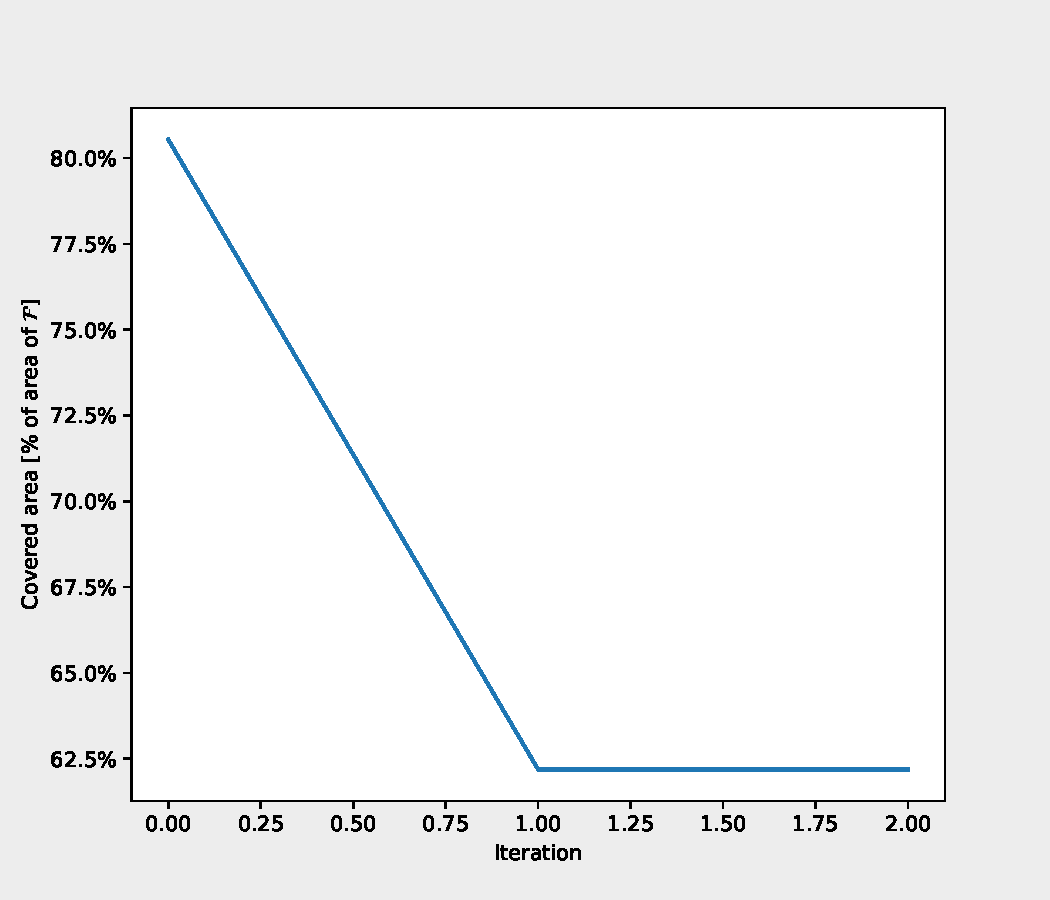
\includegraphics[width=.75\textwidth]{figs/1_by_1_center_obs_3_agnts_area_traj.pdf}
  \caption{Percentage covered  for rectangular environment with rectangular central obstacle. }
  \label[fig]{local_coverage_example}
\end{figure}
\begin{figure}[H]
  \centering
  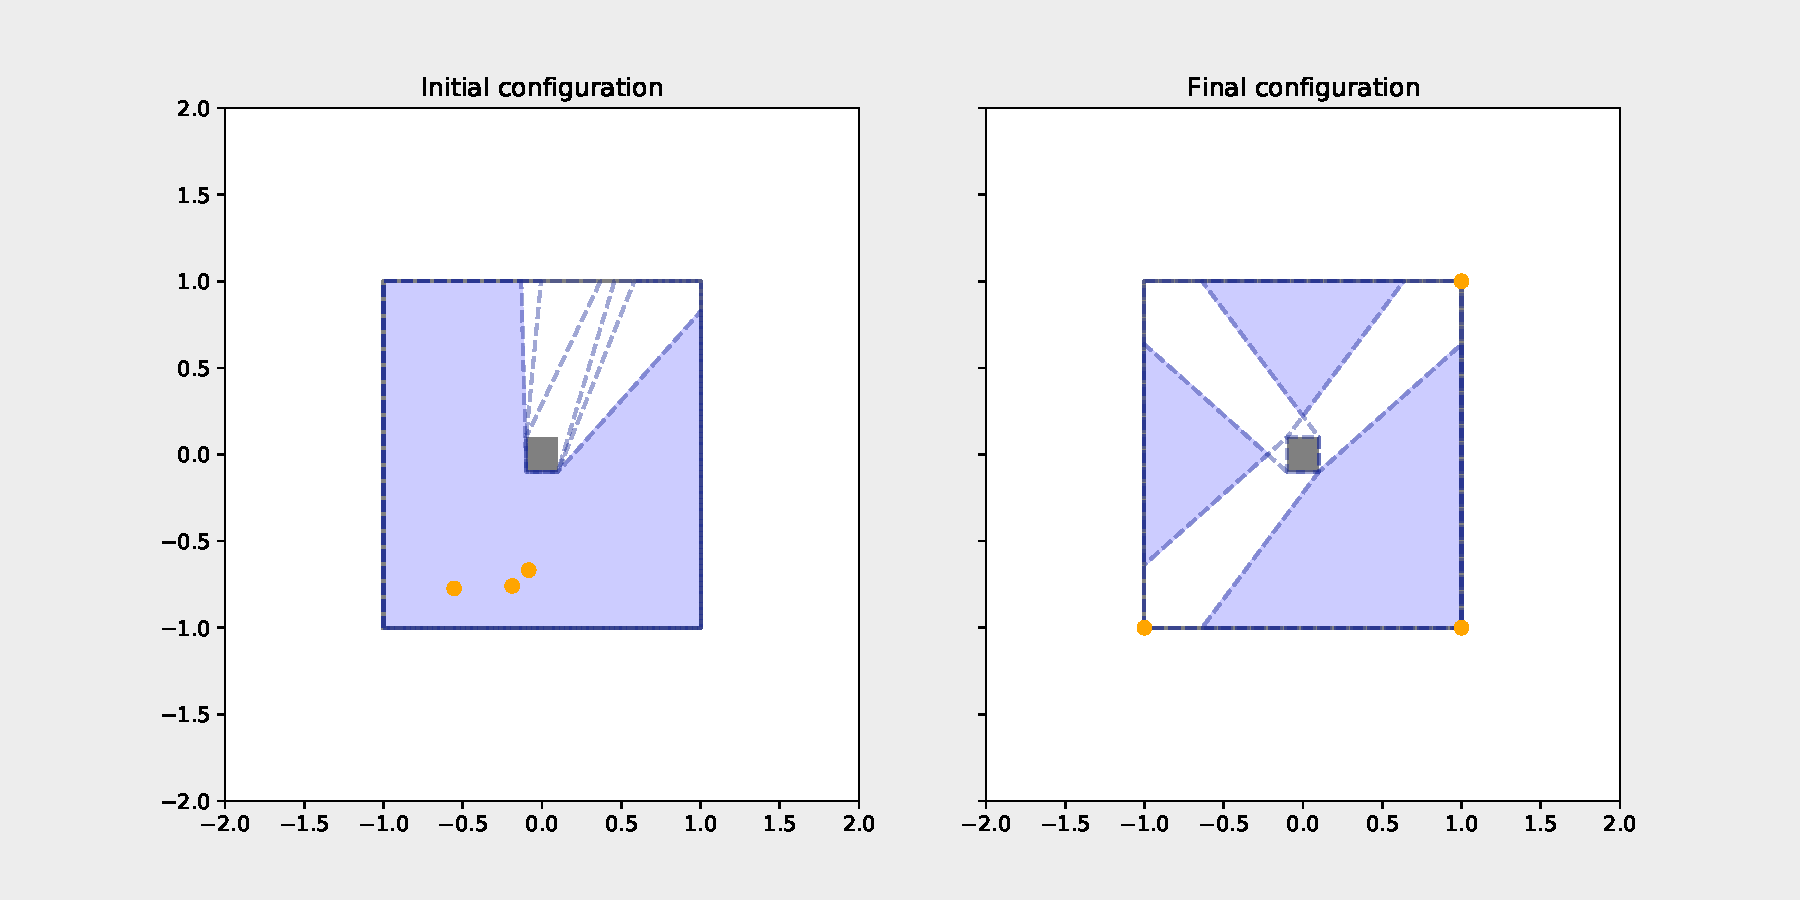
\includegraphics[width=.75\textwidth]{figs/1_by_1_center_obs_3_agnts_distr.pdf}
  \caption{Inital and final position of agents in rectangular environment with rectangular central obstacle.}
  \label[fig]{local_coverage_example}
\end{figure}

%%% 6-by-6 20 agents bottom-left obs
\begin{figure}[H]
  \centering
  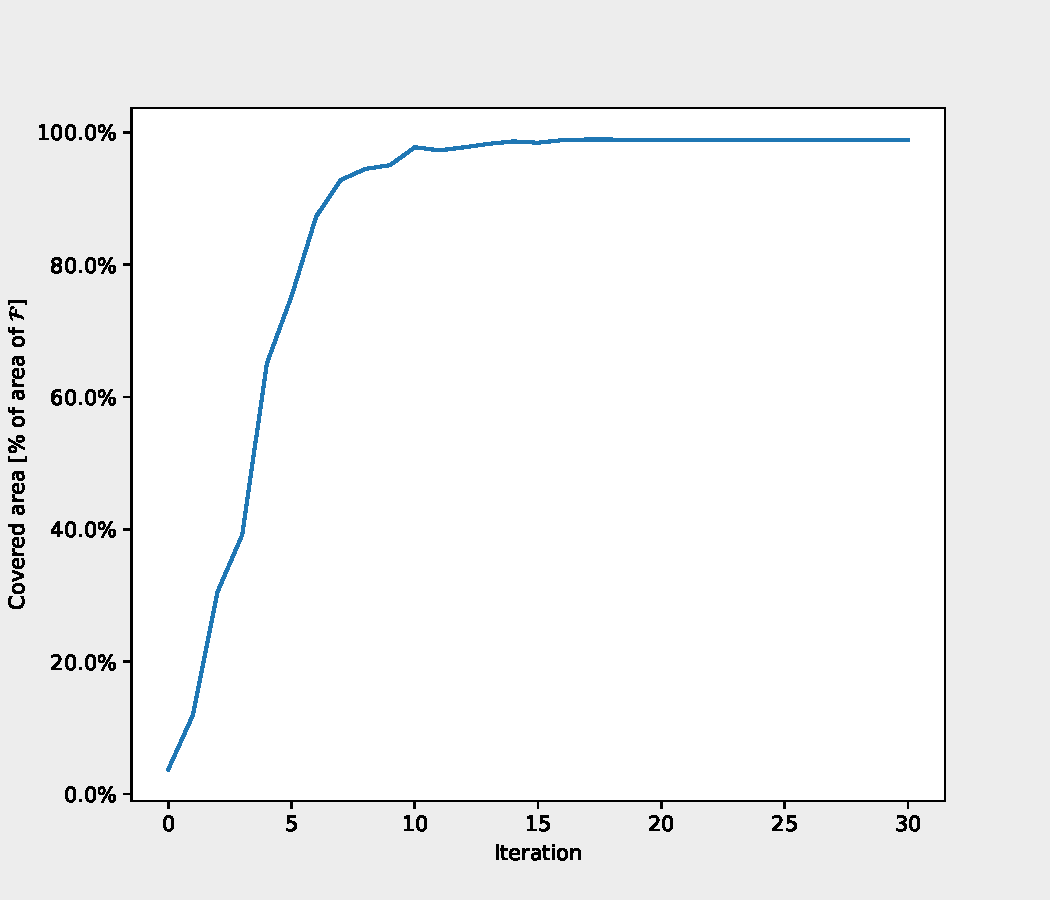
\includegraphics[width=.75\textwidth]{figs/6_by_6_bottom_left_wall_obs_20_agnts_area_traj.pdf}
  \caption{Percentage covered  for rectangular environment with blocking wall in lower left corner. }
  \label[fig]{local_coverage_example}
\end{figure}
\begin{figure}[H]
  \centering
  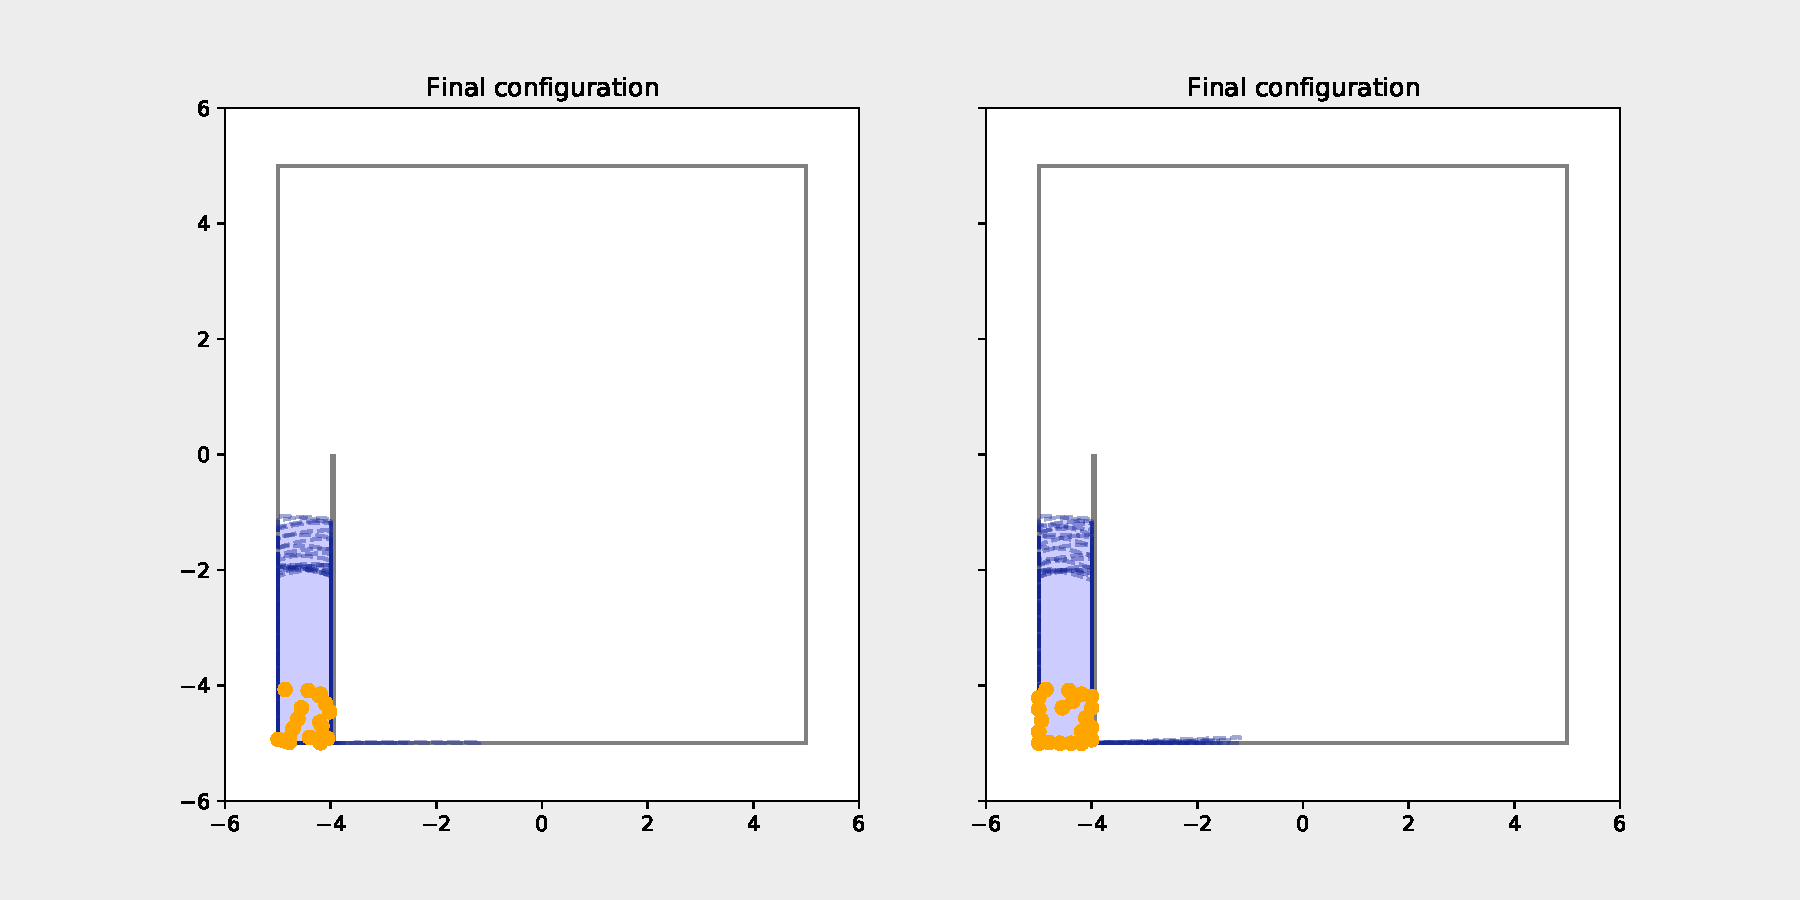
\includegraphics[width=.75\textwidth]{figs/6_by_6_bottom_left_wall_obs_20_agnts_distr.pdf}
  \caption{Inital and final position of agents in rectangular environment with blocking wall in lower left corner.}
  \label[fig]{local_coverage_example}
\end{figure}

%%% 10-by-10 21 agents hex-world
\begin{figure}[H]
  \centering
  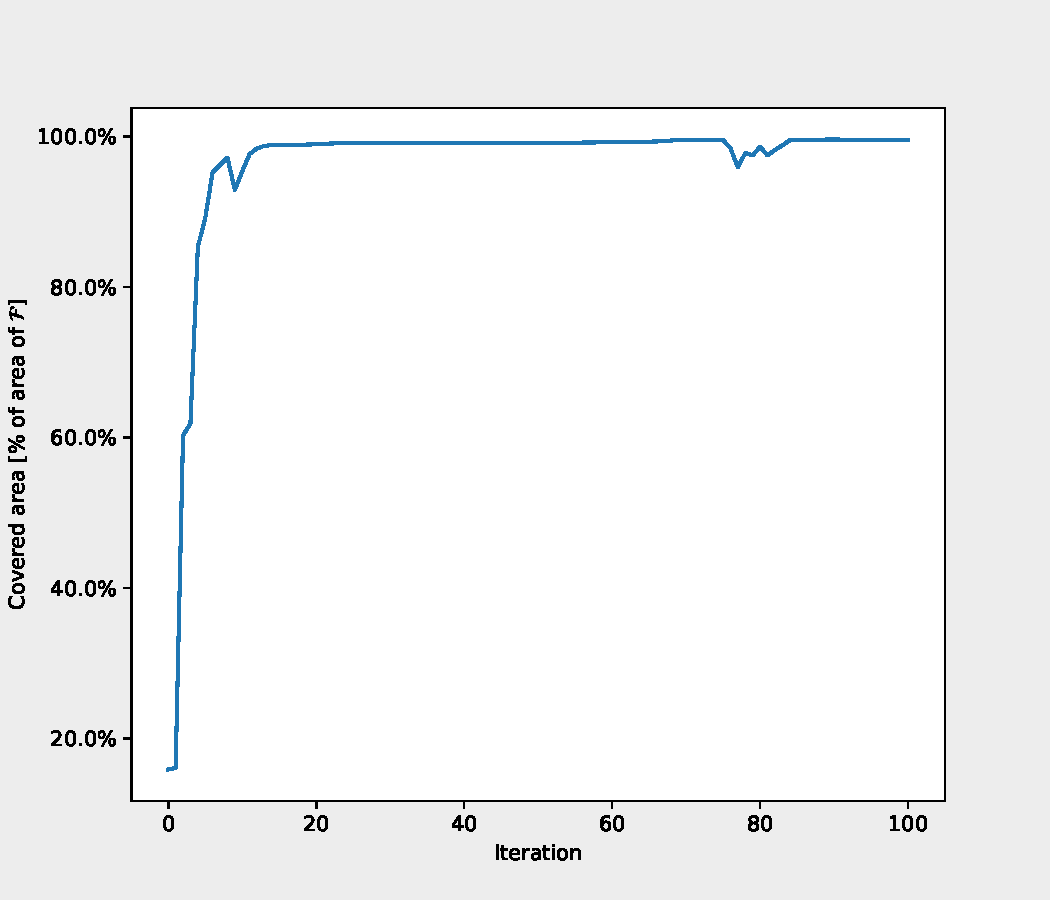
\includegraphics[width=.75\textwidth]{figs/10_by_10_hex_world_21_agnts_area_traj.pdf}
  \caption{Percentage covered for rectangular environment with blocking wall in lower left corner. }
  \label[fig]{local_coverage_example}
\end{figure}
\begin{figure}[H]
  \centering
  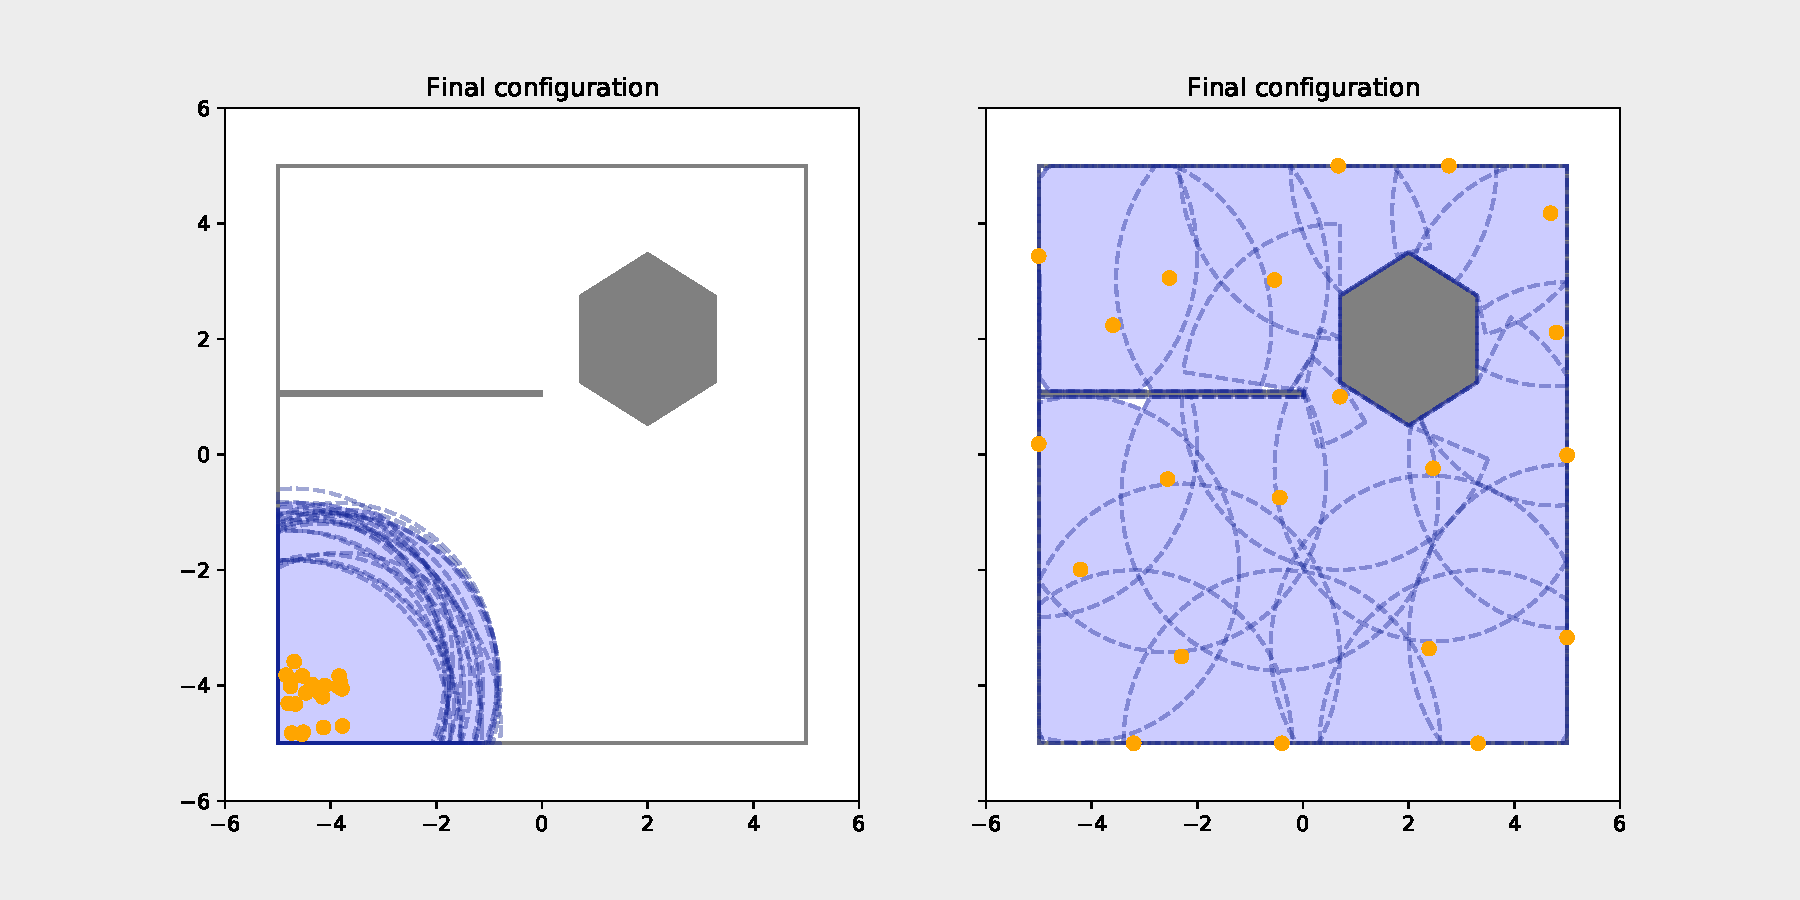
\includegraphics[width=\textwidth]{figs/10_by_10_hex_world_21_agnts_distr.pdf}
  \caption{Inital and final position of agents in rectangular environment with blocking wall in lower left corner.}
  \label[fig]{local_coverage_example}
\end{figure}